%\section{Understanding and Modeling Transient Server Preemptions}
%\section{Modeling the Dynamics of Transient Server Preemptions}
\section{Preemption Dynamics of Transient Cloud Servers}

%Understanding the nature and dynamics of transient cloud servers such as their preemption frequency is a prerequisite to understand and improve the performance of applications.

\eat{In order to understand and improve the performance of applications running on transient cloud servers, we must understand the nature and dynamics of their preemptions.
The preemption characteristics are governed by the supply of surplus resources, the demand for cloud resources, and the resource allocation policies enforced by the cloud operator.
Therefore, in this section, we present empirical and analytical models to help us understand the nature of preemptions. 
}

To measure and improve the performance of applications running on transient cloud servers, it is critical to understand the nature and dynamics of their preemptions.
The preemption characteristics are governed by the supply of surplus resources, the demand for cloud resources, and the resource allocation policies enforced by the cloud operator.
In this section, we present empirical and analytical models that describe these characteristics and enable an intuitive understanding of the nature of preemptions. 


% Transient cloud servers, by their very nature have limited availability and are frequently preempted.
% These preemptions are akin to fail-stop failures, and are often preceeded by a small advance warning (few seconds) to allow for graceful shutdowns.

% Since preemptions can impact the availability, performance, and cost of running applications, in this section, we examine their preemption characteristics.
% This modeling is important, because having a model of the availability can be useful in the context of predicting the running times of applications.
% Cloud providers offer a large number of servers of different configurations and types.
% Since transient server availability is fundamentally tied to supply and demand, the availability of servers of different types can be significantly different. 
% Thus, selecting the ``right'' server type is crucial for minimizing the overall costs. 




\subsection{The need for empirical preemption models}

Amazon's EC2 spot instances were the original cloud transient servers.
The preemptions of EC2 spot instances are based on their \emph{price}, which is dynamically adjusted based on the supply and demand of cloud resources.
Spot prices are based on a continuous second-price auction, and if the spot price increases above a pre-specified maximum-price, then the server is preempted.

Thus, the time-series of these spot prices can be used for understanding preemption characteristics such as the frequency of preemptions and the ``Mean Time To Failure'' of the spot instances.
Many research projects have used publicly available\footnotemark historical spot prices to characterize and model spot instance preemptions~\cite{spotcheck,how-to-bid}. %Add lots more here 
For example, past work has analyzed spot prices and shown that the MTTF's of spot instances of different hardware configurations and geographical zones ranges from a few hours to a few days~\cite{prateek-thesis, shastri-thesis}. 


\footnotetext{Amazon posts Spot prices of 3 months, and researchers have been collecting these prices since 2010~\cite{Buyya-prices}.}

However, Amazon has recently changed the preemption characteristics of spot instances, and servers are now preempted even if the spot price is below the maximum price.
Thus, spot prices are no longer a completely reliable indicator of preemptions, and preemptions can no longer be inferred from looking at prices alone.
Therefore, new techniques are required to model preemption dynamics that can supplement the earlier price-based approaches, and we develop these techniques next.

%\cite{alicloud-spot, packet-spot}

\subsection{Empirical preemption behavior}
%\subsection{Empirical model of preemptions}

The preemptions of transient servers need not be related to their price.
For example, Google's Preemptible VMs and Azure Batch VMs have a \emph{fixed} price relative to their non-preemptible counterparts. 
In such cases, price based models are inadequate, and other approaches to understand preemptions are required.

This task is further complicated by the fact that these cloud operators (Google and Microsoft) do not currently provide any information about preemption characteristics. 
Thus, relatively little is known about the preemptions (and hence the performance) of these transient VMs. %significantly limiting their use?

In order to understand preemption dynamics of transient servers, we conduct a large-scale empirical measurement study which is the first of its kind. 
We launched more than 1000 Google Preemptible VMs of different types over a two month period (Feb--April 2019), and measured their time to preemption (aka, their useful lifetime).\footnotemark

\footnotetext{We will release the complete preemption dataset and hope that other researchers can benefit.} %Weaksauce 


\begin{figure}
  \centering
  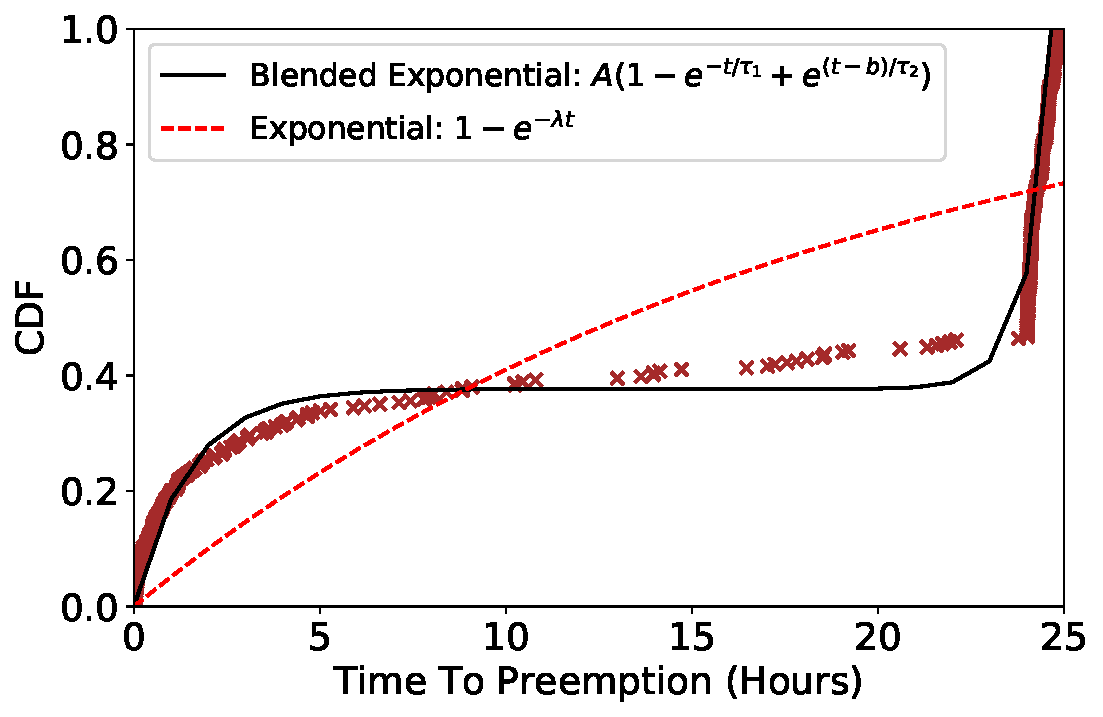
\includegraphics[width=0.4\textwidth]{../graphs/cdf_4_all.pdf}
  \caption{CDF of lifetimes of Google Preemptible Instances. Our blended exponential distribution fits much better than the conventional exponential failure distributions. }
  \label{fig:gcp1}
\end{figure}

A sample of 100 such preemption events are shown in Figure~\ref{fig:gcp1}, which shows cumulative distribution of the VM lifetimes. 
Note that the cloud operator (Google) caps the \emph{maximum} lifetime of the VM to 24 hours, and all the VMs are preempted before that hard limit.
Furthermore, the lifetimes of VMs are \emph{not} uniformly distributed, but have three distinct phases. 
In the first phase, characterized by VM lifetime $t\in (0,3)$ hours, we observe that many VMs are quickly preempted after they are launched, and thus have a steep rate of failure initially; the rate of failure or preemptions can be obtained by taking the derivative of the CDF. The second phase characterizes the VMs that survive past 3 hours and enjoy a relatively low and uniform preemption rate over a relatively broad range of lifetime (characterized by the slowly rising CDF in Figure~\ref{fig:gcp1}). The final phase exhibits a steep increase in the number of preemptions as the preemption deadline of 24 hours approaches. The overall rate of preemptions is ``bath tub'' shaped.
%\it I think we should show the probability plot to exhibit the bath tub shape

%The preemption rate is ``bath tub'' shaped, with VMs that survive past 3 hours enjoying a relatively low preemption rate, and finally a steep increase in the number of preemptions as the preemption deadline (24 hours) approaches. 

We note that this preemption behavior, imposed by the constraint of the small, 24 hour  lifetime, is \emph{substantially} different from conventional failure characteristics of hardware components and even EC2 spot instances.
In these ``classical'' setups, the rate of failure  usually follows an exponential distribution $f(t) = \lambda e^{-\lambda t}$, where $\lambda=1/\text{MTTF}$.
Figure~\ref{fig:gcp1} shows the CDF ($=1-e^{-\lambda t}$) of the exponential distribution when fitted to the observed preemption data, by finding the distribution parameter $\lambda$ that minimizes the least squares error.
From Figure~\ref{fig:gcp1}, we can see that the classic exponential distribution is unable to model the observed preemption characteristics.
%The primary reason is that the exponential distribution assumes that the \vj{the rate of preemptions is independent of the lifetime of the VMs} (preemptions are \emph{memoryless}), which does not hold true when there is a fixed upper bound on the lifetime, as is the case for Google Preemptible VMs. \vj{In other words, the conventional approach is insufficient to model constrained preemption dynamics.}
We attribute this deficiency to the central assumption made in the underlying reliability theory principles that leads to the exponential distribution: the rate of preemptions is independent of the lifetime of the VMs, in other words, the preemptions are \emph{memoryless}.
This assumption breaks down when there is a fixed upper bound on the lifetime, as is the case for Google Preemptible VMs, and the conventional approach becomes insufficient to model this constrained preemption dynamics. 

\subsection{Analytical model of preemption dynamics in Google cloud}

We now develop a \emph{minimal} analytical model for preemption dynamics that is faithful to the empirically observed data and provides a basis for developing running-time and cost-minimizing optimizations presented in Section~\ref{sec:design}.
This new model is based on the earlier observation that the cumulative distribution of lifetimes has multiple distinct temporal phases. The key assumption underlying our minimal model is the presence of two distinct failure processes that give rise to a new probability distribution characterizing the preemptions and the observed CDF, and ensure the dependence of the rate of failure on the VM lifetime. The first process dominates over the initial temporal phase and yields the classic exponential distribution that captures the steep rate of early preemptions. The second process dominates over the final phase near the 24 hour maximum VM lifetime and is assumed to be characterized by an exponential term that captures the sharp rise in preemptions that results from the constraint of a fixed 24 hour lifetime. Generally, these two processes compete during the middle phase to yield a relatively constant and low number of preemptions; in practice, based on the fits to the empirical data, we observe the first process to dominate over the second during this phase as well. 

%The first two phases are reasonably captured by the classic exponential distribution. In order to model the overall observed empirical CDF, we add another term that captures the failure process near the 24 hour maximum VM lifetime,  and construct a \emph{new} probability distribution. 
%
%we develop a \emph{new} probability distribution that is composed by blending two failure processes that act on different temporal phases over the 24 hour maximum lifetime of the VMs. 
%
%We write the general form of our blended preemption CDF as follows:

We propose the following general form for the CDF based on this model:
\begin{equation}
  \label{eq:blend1}
  \mathscr{F}\left(t\right) = A\left(1-e^{-\frac{t}{\tau_1}} + e^{\frac{t-b}{\tau_2}}\right),
\end{equation}
where $1/\tau_1$ is the rate of preemptions in the initial phase, $1/\tau_2$ is the rate of preemptions in the final phase (generally, $1/\tau_2 > 1/\tau_1$), $b$ denotes the time when the preemptions occur at a high rate (generally, around 24 hours) which we term the activation time for the second process, and $A$ is a constant used to scale the CDF to ensure that the initial conditions ($F(0)=0$) are met.

For most of its life, a VM sees failures according to the classic exponential distribution with a rate of failure equal to $1/\tau_1$ -- this behavior is captured by $1-e^{-t/\tau_1}$ term in Eq.~\ref{eq:blend1}. 
%However, this does not capture the finite lifetime of the VM imposed by the cloud operator.
As VMs get closer to their maximum lifetime (24 hours) imposed by the cloud operator, they are reclaimed (i.e., preempted) at a high, exponential rate, which is captured by the second term introduced in the CDF ($e^{(t-b)/\tau_2}$). 
Shifting the argument ($t$) of the exponential by $b$ ensures that the exponential reclamation is only applicable towards the end of the VM's maximum lifetime and does not dominate over the entire temporal range. As noted before, $1/\tau_2$ is the rate of this reclamation.

The analytical model and the associated 4 parameter distribution function $\mathscr{F}$ introduced above provides a much better fit to the empirical data and captures the different phases of the preemption dynamics through parameters $\tau_1, \tau_2, b$, and $A$. These parameters characterizing the preemption dynamics can be obtained for a given empirical CDF by minimizing least-squared function fitting methods. \footnotemark 
%
\footnotetext{More details about the distribution fitting are presented in the implementation section(~\ref{sec:impl}}
%
In the next section, we use this analytical model for optimizing cloud resource selection such that we can run scientific applications at low cost and running times. We note that our motivation here is to provide a minimal model, i.e. a model based on data-driven observations and reasonable assumptions that provides a sufficiently accurate description of constrained preemption dynamics with the minimal number of necessary parameters. As is evident from Figure.~\ref{fig:gcp1}, the analytical $\mathscr{F}$ shows deviations from the data near the halfway point within the 24 hour lifetime. One can envision generalizing this model by including more failure processes characterized by failure rates and activation times (like $b$) to capture the data with higher accuracy. Of course, this introduces a higher number of parameters and reduces the predictive power and simplicity of the model. 


\subsection{Preemption dynamics of VMs of different types}
\label{subsec:types-dynamics}
%%%%%%%%%%%%%%%%%%%% OPTIONAL
Since cloud platforms support a wide range of applications, they also offer a large range of servers (VMs) with different resource configurations (such as the number of CPU cores, memory size, I/O bandwidths, etc.). 
For example, a cloud provider may offer VMs with (4 CPUs, 4 GB memory), (8 CPUs, 8 GB memory), etc.
Most clouds offer a large number of different hardware configurations---Amazon EC2 offers more than 50 hardware configurations, for example~\cite{amazon-ec2-instance-types}.

\begin{figure}
  \centering 
  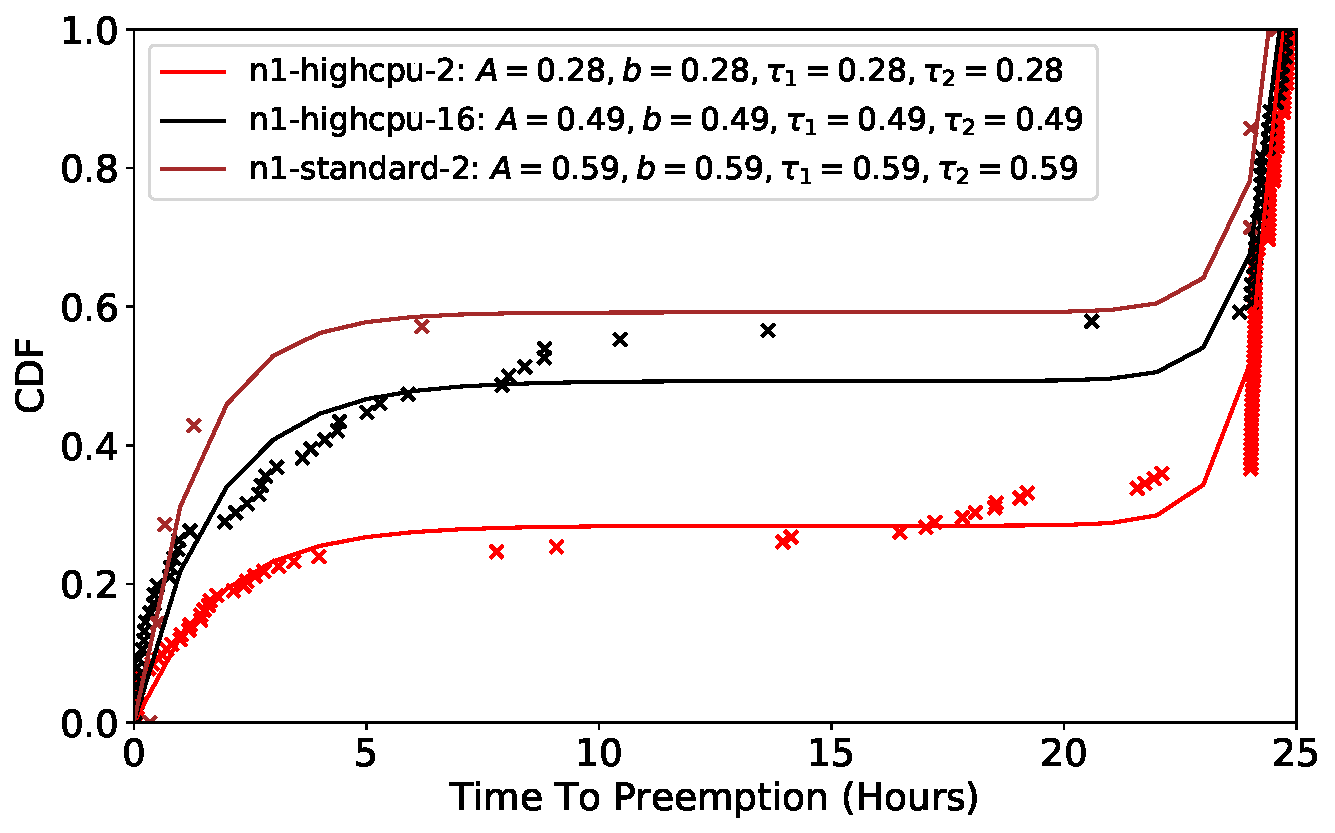
\includegraphics[width=0.4\textwidth]{../graphs/cdf_comparison_3.pdf}
  \caption{The preemption characteristics of different VM types. Larger VMs are more likely to be preempted}
  \label{fig:cdf-comparison}
\end{figure}

In general, the preemption dynamics of a VM are determined by the supply and demand of VMs of that \emph{particular} type.
Thus, the preemption characteristics of VMs of different sizes and running in different geographical zones are different.
Figure~\ref{fig:cdf-comparison} shows the preemption CDF's of three such VM types in the Google Cloud, along with the parameters of our four parameter distribution.
We show the data from three different types of VMs \texttt{n1-highcpu-\{2,8,32\}}, where the number indicates the number of CPU's. 

From Figure~\ref{fig:cdf-comparison}, we see that our distribution is able to capture the preemption dynamics of different VM types.
Interestingly, we can also observe that larger VMs have a higher rate of failure.
This is because larger VMs require more computational resources (such as CPU and memory), and when the supply of resources is low, the cloud operator can reclaim a large amount of resources by preempting larger VMs.
This observed behavior aligns with the guidelines for using preemptible VMs that suggests the use of smaller VMs when possible~\cite{gcp-preempt-faq}. 


Our analytical model also helps use crystallize the differences in VM preemption dynamics, by allowing us to easily calculate their expected lifetime. 
More formally, we define the expected lifetime of a VM of type $i$, as 
\begin{equation}
  \label{eq:expected-lifetime}
E[L_i] =  \int_{0}^{24} t {f_i}(t)~dt 
\end{equation}
Where $f(t) = \dfrac{d \mathscr{F}(t)} {dt} = A \left(\dfrac{1}{\tau_1}e^{-t/\tau_1} + \dfrac{t-b}{\tau_2}e^{\frac{t-b}{\tau_2}}\right) $ 

Since preemptions require restarting a job and increase the job completion time, it may be more prudent to select transient VMs with higher expected lifetimes. We use the analytically derived expected lifetimes of VMs of different types in \sysname when selecting the the ``best'' VM type for a given bag of jobs. This server selection is a key part of \sysname design, which we describe next. 

% \subsection{EC2 spot instances}

% The earliest form of transient cloud instances.
% In addition to having dynamic availability, also have dynamic pricing.
% ``Classic'' spot instances had price determining the availability, and thus a large amount of work was devoted to bidding and analyzing the prices.

% However a recent change to the spot prices no longer allows these assumptions, rendering it impossible to obtain the \emph{exact} availability information from the prices alone.


% \subsection{Google Preemptible VMs}

% Launched in 2015.
% Flat-rate discount of 80\% compared to on-demand servers.
% Interesting availability SLA: the maximum lifetime is 24 hours, and can be preempted earlier as well.

% In this paper we will look at these preemptible VMs and show how to model their availability.
% Given the inability to use EC2 prices, we believe that our approach is more generalizable and robust.


% There are some distinguishing characteristics of GCP preemptible VMs that makes their failure modeling challenging.
% First is their flat pricing and no other signalling information about their preemption rates (MTBFs) that makes server selection difficult.

% \textbf{Modeling Failure Behavior of Preemptible VMs}
% CDF is ``sigmoid'' shaped.
% $P=R*np.sinh((t-t0)/tau) + C$ with a very low $R=10^{-6}, t_0=12, \tau=0.9, C=0.36$

% Basically, this is a mixture of two distributions, the standard exponential distribution, which we call the stabilization rate and an exponentially increasing reclamation rate.

% Preemptible VMs have three availability phases.

% There are many early deaths, then a period of low failure rates, and then the failure rate is exponential with a positive exponent to enable the cloud provider to reclaim the VMs within the deadline (24 hours in the case of Google's Preemptible VMs).








%%% Local Variables:
%%% mode: latex
%%% TeX-master: "paper"
%%% End:
